%--------------------------------------------CAPA DE APLICACIÓN ------------------------------------------------------%

\subsection{Capa de aplicación}

Los elementos de la capa de aplicación se utilizan normalmente para modelar la arquitectura de la aplicación que describe la \textbf{estructura, el comportamiento y la interacción de las aplicaciones de la empresa}.

La tabla \ref{tab:Tabla de la capa de aplicación}  ofrece una descripción general de los elementos de la capa de aplicación, con sus definiciones.\cite{archimate} 


\begin{longtable}{|p{0.15\linewidth}|p{0.45\linewidth}|p{0.2\linewidth} p{0.2\linewidth}|}
    \caption{Tabla de la capa de aplicación}
    \\
    \hline
    \rowcolor[HTML]{AFC5F6} 
    \textbf{Elemento} & \textbf{Descripción} & \multicolumn{2}{c|}{\textbf{Notación}} \\
    \hline
    \endhead
    \hline
    \multicolumn{4}{r}{\textit{Continúa en la siguiente página}} \\
    \endfoot
    \hline
    \endlastfoot
    \label{tab:Tabla de la capa de aplicación}
    %Contenido 1 &
    %\lipsum[1] &
    %Datos A1
    %& Datos B1
    %\\
    %\hline



    Componente de Aplicación 
    &
    Representa una parte modular, reemplazable y desplegable de un sistema de software que encapsula su comportamiento y datos. 
    &
\begin{center}
    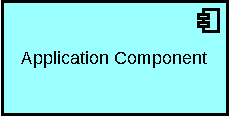
\includegraphics[width=1\linewidth]{imgs/capa_aplicacion/aplication_component.pdf}
\end{center} 
&
\begin{center}
    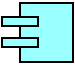
\includegraphics[width=0.5\linewidth]{imgs/capa_aplicacion/component.pdf}
\end{center}
    \\ \hline



    Colaboración de Aplicación 
    &
    Indica una unidad de comportamiento colectivo que agrupa componentes de aplicación para ofrecer una funcionalidad empresarial conjunta. 
    &
\begin{center}
    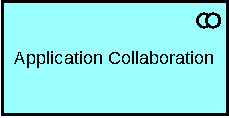
\includegraphics[width=1\linewidth]{imgs/capa_aplicacion/Aplication_collaboration.pdf}
\end{center} &
\begin{center}
    
\includegraphics[width=0.7\linewidth]{imgs/capa_aplicacion/collaboration.pdf}
\end{center}
    \\ \hline



    Interfaz de Aplicación 
    &
    Representa un punto de acceso en el que los servicios de la aplicación se ponen a disposición de un usuario, otro componente de la aplicación o un nodo. 
    &
\begin{center}
    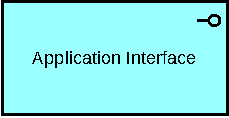
\includegraphics[width=1\linewidth]{imgs/capa_aplicacion/Aplication_interface.pdf}
\end{center} &
\begin{center}
    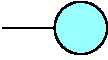
\includegraphics[width=0.7\linewidth]{imgs/capa_aplicacion/interfaz.pdf}
\end{center}
    \\ \hline



    Función de Aplicación 
    &
    Representa el comportamiento automatizado que puede realizar un componente de la aplicación. 
    &
\begin{center}
    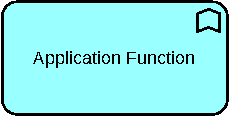
\includegraphics[width=1\linewidth]{imgs/capa_aplicacion/Aplication_function.pdf}
\end{center} &
\begin{center}
    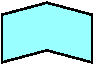
\includegraphics[width=0.7\linewidth]{imgs/capa_aplicacion/function.pdf}
\end{center}
    \\ \hline

    Interacción de Aplicación 
    &
    Representa una unidad de comportamiento colectivo de la aplicación realizada por (una colaboración de) dos o más componentes de la aplicación. 
    &
\begin{center}
    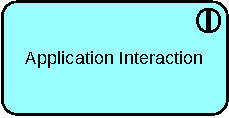
\includegraphics[width=1\linewidth]{imgs/capa_aplicacion/Aplication_interaction.pdf}
\end{center} &
\begin{center}
    
\includegraphics[width=0.7\linewidth]{imgs/capa_aplicacion/interaction.pdf}
\end{center}
    \\ \hline

    Proceso de Aplicación 
    &
    Representa una secuencia de comportamientos de la aplicación que logra un resultado específico. 
    &
\begin{center}
    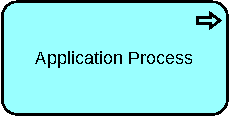
\includegraphics[width=1\linewidth]{imgs/capa_aplicacion/aplication_process.pdf}
\end{center} &
\begin{center}
    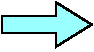
\includegraphics[width=0.7\linewidth]{imgs/capa_aplicacion/process.pdf}
\end{center}
    \\ \hline

    Evento de Aplicación 
    &
    Representa un cambio de estado de la aplicación. 
    &
\begin{center}
    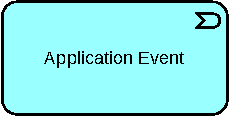
\includegraphics[width=1\linewidth]{imgs/capa_aplicacion/Aplication_event.pdf}
\end{center} &
\begin{center}
    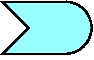
\includegraphics[width=0.7\linewidth]{imgs/capa_aplicacion/event.pdf}
\end{center}
    \\ \hline


    Servicio de Aplicación 
    &
    Representa un comportamiento de aplicación expuesto definido explícitamente. 
    &
\begin{center}
    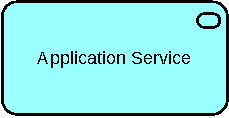
\includegraphics[width=1\linewidth]{imgs/capa_aplicacion/Aplication_service.pdf}
\end{center} &
\begin{center}
    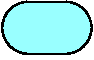
\includegraphics[width=0.7\linewidth]{imgs/capa_aplicacion/service.pdf}
\end{center}
    \\ \hline

    
    Objeto de Datos 
    &
    Representa datos estructurados para su tratamiento automatizado. 
    &
\begin{center}
    \includegraphics[width=1\linewidth]{imgs/capa_aplicacion/aplication_dataObject.pdf}
\end{center} &
\begin{center}
    \includegraphics[width=0.7\linewidth]{imgs/capa_aplicacion/Data_object.pdf}
\end{center}
    \\ \hline
\end{longtable}